\documentclass{beamer}

\usepackage{beamerthemesplit}
\usetheme{Singapore} 

\input{../../include/preamble.inc} 
\input{../../include/definitions.inc} 
\input{../../include/author.inc} 

\title[]{Сильные разрывы в сплошной среде}

\begin{document}
	
\frame[plain]{\titlepage}


\frame[plain]{
	\frametitle{Аннотация}
	\parbox{\textwidth}{
		Обобщённые движения сплошной среды. Соотношения на сильном скачке. Классификация сильных разрывов. Соотношение для ударных волн.
	}
}

\frame{
	\frametitle{ Законы сохранения в дивергентной форме }
	
	\[
		\displaystyle\pd{\rho}{t} + \operatorname{div} (\rho \vec{v})  =  0, 
	\]
	\[
		\displaystyle\pd{\rho\vec{v}}{t} + \operatorname{div} (\rho\vec{v}\otimes\vec{v} - \sigma) =  0, 
	\]
	\[
		\displaystyle\pd{}{t} \left( \rho \left(\varepsilon + \frac{\vec{v}^2}{2} \right) \right)
		+ \operatorname{div}\left( \rho \left(\varepsilon + \frac{\vec{v}^2}{2} \right) \vec{v} - \sigma\cdot \vec{v} + \vec{q} \right)  = 0.
	\]

	\medskip
	\begin{exampleblock}{Обобщенная форма записи}
		\parbox{\textwidth}{
			Каждый из этих законов можно записать в следующем виде, который представляет собой дивергенцию вектора в 4-х мерном пространстве относительно $\argtxv$:
			
			\[
				\pd{f}{t} + \operatorname{div} (f\vec{v}+\vec{\varphi}) = 0.
			\]
		}
	\end{exampleblock}


}

\frame{
	\frametitle{ Обобщённые движения }
	
	\begin{exampleblock}{ Интеграл в четырёхмерном пространстве}
		\parbox{\textwidth}{
			
			Рассмотрим $\Omega \subset R^4 $ -- ограниченная область с кусочно-гладкой границей $\Gamma$ и сечениями $\omega_{\Omega}(t)$ гиперплоскостями при $t=const$. Интегралы по $\Omega$ от законов сохранения в дивергентной форме имеют вид
			\[
			\int\limits_{t_1}^{t_2} \int\limits_{\omega_{\Omega}(t)} (f_t + \operatorname{div}(f\vec{v} + \vec{\varphi})) d\omega dt = 0.
			\]
			
		}
	\end{exampleblock}
	

}


\frame{
	\frametitle{ Обобщённые движения }
		\begin{exampleblock}{ Слабая форма записи }
		\parbox{\textwidth}{
			Согласно теореме Гаусса-Остроградского для вектора $\vec{g} = (f, f v_1+\varphi_1,  f v_2+\varphi_2, f v_3+\varphi_3)$ имеет место
			\[
			\int\limits_\Gamma \vec{g} \cdot \vec{\nu} d\Gamma = 0,
			\]
			где $\vec{\nu} = \vec{l} \cos(\vec{\nu},t) + \vec{n} \sin (\vec{\nu},t)$ -- нормаль к $\Gamma$ в четырёхмерном пространстве; $\vec{l}$ -- орт оси $t$,
			$\vec{n}$ -- орт внешней нормали к сечению $\Gamma$ гиперплоскостью $t=const$.
			 
			
			
		}
	\end{exampleblock}
}

\frame{
	\frametitle{ Обобщенные движения }

	\begin{exampleblock}{Интегральная форма записи }
		\parbox{\textwidth}{
			Т.к. 
			\[
			\vec{g} \cdot \vec{\nu} = f \cos(\vec{\nu},t) + (f\vec{v}+\vec{\varphi})\cdot \vec{n} \sin (\vec{\nu},t),
			\]
			то
			\[
			\int\limits_\Gamma \left(
			f \cos(\vec{\nu},t) + (f\vec{v}+\vec{\varphi})\cdot\vec{n} \sin (\vec{\nu},t)
			\right)
			d\Gamma = 0.
			\]
			
		}
	\end{exampleblock}


}

\frame{
	\frametitle{ Обобщённое движение сплошной среды}
	\begin{exampleblock}{Определение}
	\parbox{\textwidth}{
			Набор функций $\rho$, $\vec{v}$, $\sigma$, $\varepsilon$, определённых в $R^4\argtxv$ называется \alert{обобщённым движением} сплошной среды, если для любой замкнутой кусочно-гладкой поверхности $\Gamma \subset R^4\argtxv$ эти функции удовлетворяют соотношениям
			\small
			\[
			\int\limits_\Gamma \left(
			\rho \cos(\vec{\nu},t) + \rho\vec{v} \cdot\vec{n} \sin (\vec{\nu},t)
			\right) \. d\Gamma = 0,
			\]
			\[
			\int\limits_\Gamma \left(
			\rho\vec{v} \cos(\vec{\nu},t) + (\rho\vec{v}\otimes\vec{v}-\sigma)\cdot\vec{n} \sin (\vec{\nu},t)
			\right) \. d\Gamma = 0,
			\]
			\[
			\int\limits_\Gamma \left(
			 \rho \left(\varepsilon + \frac{\vec{v}^2}{2} \right) \cos(\vec{\nu},t) +
			\left(
			 \rho \left(\varepsilon + \frac{\vec{v}^2}{2} \right) \vec{v} - \sigma\cdot \vec{v} +
			 \vec{q} 
			\right)
			\cdot\vec{n} \sin (\vec{\nu},t) 
			\right) \. d\Gamma	=
			\]
			\[
			=0.
			\]
			
%				\displaystyle\pd{}{t} \left( \rho \left(\varepsilon + \frac{\vec{v}^2}{2} \right) \right)
%			+ \operatorname{div}\left( \rho \left(\varepsilon + \frac{\vec{v}^2}{2} \right) \vec{v} - \sigma\cdot \vec{v} + \vec{q} \right)  = 0.
	}
	\end{exampleblock}
	
}

\frame{
	\frametitle{ Движение с сильным разрывом }
	
	\begin{exampleblock}{Определение}
		\parbox{\textwidth}{
			Если в области определения обобщённого движения существует гиперповерхность $\Sigma \subset R^4$, на которой величины $\rho$, $\vec{v}$, $\sigma$, $\varepsilon$ имеют разрыв первого рода и вне которой это движение гладкое, то такое движение называется \alert{движением с сильным разрывом}, а сечение $B(t)$ гиперповерхности  $\Sigma$ гиперплоскостями $t=const$ называется поверхностью сильного разрыва.
		}
	\end{exampleblock}

	\begin{exampleblock}{Сильные разрывы}
		\parbox{\textwidth}{
			Величины разрывов (скачков) не могут быть произвольными, а должны удовлетворять уравнениям сильного разрыва, которые следуют из уравнений обобщённого движения.
		}
	\end{exampleblock}
	
}

\frame{
	\frametitle{ Соотношения на сильном скачке }
	
	\begin{columns}
		\begin{column}{0.65\textwidth}
			\parbox{\textwidth}{
				Рассмотрим временной интервал $[t_1, t_2]$, на котором существует разрыв функции $\Sigma$. Для каждого $t$ рассмотрим небольшую окрестность разрыва в $R^3$ высоты $2h$. Тогда для этой области можно записать закон сохранения в общем виде
				\[
				\int\limits_\Gamma \left(
				f \cos(\vec{\nu},t) + (f\vec{v}_n+\vec{\varphi}_n) \sin (\vec{\nu},t)
				\right)
				d\Gamma = 0.	
				\]
				
				Интеграл по $\Gamma$ разбивается на $3$ интеграла по поверхностям $S_1$, $S_2$, параллельным гиперповерхности разрыва $\Sigma$  и боковой поверхности $S_3$. 
			}
		\end{column}
		\begin{column}{0.35\textwidth}
			\centering
			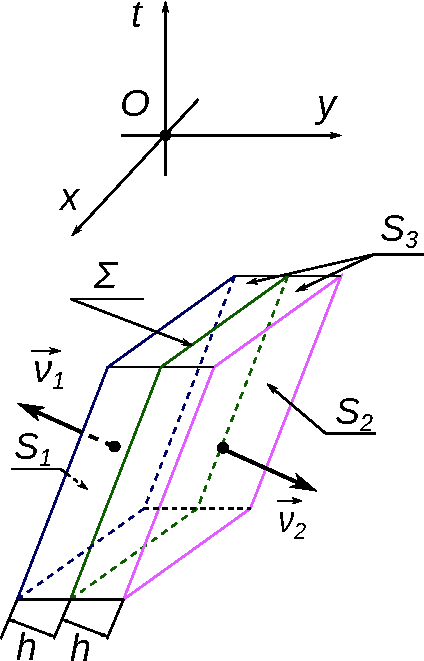
\includegraphics[width=\textwidth]{../img/jump2.pdf}
		\end{column}
	\end{columns}
	
}

\frame{
	\frametitle{ Соотношения на сильном скачке }
	
	\begin{columns}
		\begin{column}{0.65\textwidth}
			\parbox{\textwidth}{
				При $h \to 0$ интеграл по поверхности $S_3$	будет стремиться к $0$,
				а интегралы  по $S_1$ и $S_2$ -- к интегралам от параметров среды справа и слева от гиперповерхности разрыва, при этом $\vec{\nu}_1=-\vec{\nu}_2$.
			
				\medskip
				В силу произвольности выбранных $S_1$ и $S_2$ и непрерывности подынтегральных выражений слева и справа от разрыва получится выражение
				\[
				[f \cos(\vec{\nu},t) + (f\vec{v}_n+\vec{\varphi}_n) \sin (\vec{\nu},t)] = 0,
				\]
				где $[a] = a_2-a_1$ -- скачок величины $a$ на разрыве.
				

			}
		\end{column}
		\begin{column}{0.35\textwidth}
			\centering
			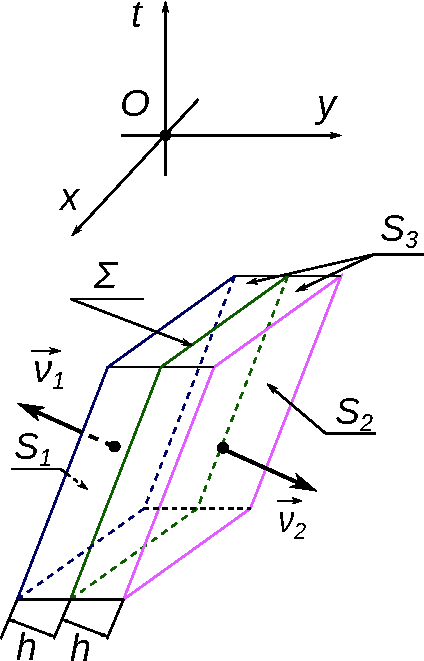
\includegraphics[width=\textwidth]{../img/jump2.pdf}
		\end{column}
	\end{columns}
	
}

\frame{
	\frametitle{ Соотношения на сильном скачке }
	
	\begin{exampleblock}{Определение }
		\parbox{\textwidth}{
			Скоростью перемещения поверхности разрыва $B(t)$ в точке $M$ называется предел
			\[
			D_n(M) = \lim_{t \to 0 }\frac{H(M,t, \delta t)}{\delta t},
			\]
			где $H(M,t,\delta t)$ --  расстояние, на которое переместилась поверхность вдоль нормали $\vec{n}$, выпущенной из заданной точки поверхности разрыва $M$ в момент времени $t$. $D_n$ принимает отрицательные значения, если движение направлено в противоположную сторону $\vec{n}$.
		}
	\end{exampleblock}


	
}

\frame{
	\frametitle{  Соотношения на сильном скачке }
	
	
	\begin{exampleblock}{Свойство}
	\parbox{\textwidth}{
		Вектор 
		\[
		D_n \vec{n}+\vec{l}
		\]
		является касательным вектором к гиперповерхности $\Sigma$, потому что точка $M$ за время $\delta t$ переместится на вектор $H(M,t, \delta t) \delta t \,\vec{n}+\delta t \, \vec{l}$.
	}
	\end{exampleblock}
	
	\begin{exampleblock}{Связь вектора $\vec{\nu}$ и скорости $D_n$}
		\parbox{\textwidth}{

			Вектор	$D_n \vec{n}+\vec{l}$ ортогонален вектору $\vec{\nu} = \vec{l} \cos(\vec{\nu},t) + \vec{n} \sin (\vec{\nu},t)$, нормали к гиперповерхности $\Sigma$,  таким образом
			\[
				( \cos(\vec{\nu},t) \, \vec{l} +  \sin (\vec{\nu},t) \, \vec{n} )\cdot
				(D_n \, \vec{n}+\vec{l}) = D_n \sin(\vec{\nu},t) + \cos(\vec{\nu},t)=0
			\]
			и
			\[
			D_n = - \cos(\vec{\nu},t)/\sin(\vec{\nu},t).
			\]
		}
	\end{exampleblock}
}

\frame{
	\frametitle{ Соотношения на сильном скачке }
	
	\begin{exampleblock}{В общем виде }
		\parbox{\textwidth}{
			С учётом связи $D_n = - \cos(\vec{\nu},t)/\sin(\vec{\nu},t)$
			\[
			[f(v_n - D_n) + \varphi_n] = 0.
			\]
		}
	\end{exampleblock}

	\begin{exampleblock}{\alert{Уравнения Гюгонио} в газовой динамике}
		\parbox{\textwidth}{
			Положив в исходных уравнениях $\sigma = -pI$, $\vec{q} = \vec{0}$, получим в результате подстановки выражений для $f$ и $\varphi$ из законов сохранения соотношения
			\[
			\left[
			\rho(v_n-D_n)
			\right] = 0,
			\]
			\[
			\left[
			\rho\vec{v}(v_n-D_n) + p \vec{n} 
			\right] = 0,
			\]
			\[		
			\left[
			\rho \left(\varepsilon + \frac{\vec{v}^2}{2} \right) (v_n - D_n) +p v_n
			\right] = 0.
			\]
		}
	\end{exampleblock}
	
}

\frame{
	\frametitle{ Классификация сильных разрывов }
	
	\begin{exampleblock}{Определения}
		\parbox{\textwidth}{
			Обозначим $m = \rho (u_n - D_n)$ -- масса вещества, проходящее через поверхность разрыва. Обозначим $v_\tau$ -- составляющая скорости, лежащая в касательной плоскости к поверхности разрыва.
			
		}
	\end{exampleblock}

	\pause
	
	\begin{exampleblock}{Контактный разрыв ($m = 0$)}
		\parbox{\textwidth}{
			\begin{itemize}
				\item  $[p]=0$ и $[u_n]$ = 0,
				\item  $[\rho] \neq 0$,  $[\varepsilon] \neq 0$, $v_{\tau} \neq 0$.
			\end{itemize}
			
		}
	\end{exampleblock}

	\pause

	\begin{exampleblock}{Ударная волна ($m \neq 0$)}
		\parbox{\textwidth}{
		\begin{itemize}
			\item  $[u_{\tau}]$ = 0,
			\item  $[p] \neq 0$, $[\rho] \neq 0$,  $[\varepsilon] \neq 0$, $v_{n} \neq 0$.
		\end{itemize}	
		}
	\end{exampleblock}
	
}

\frame{
	\frametitle{ Соглашение для ударных волн }
	\begin{exampleblock}{Определение}
		\parbox{\textwidth}{
			Поверхность ударной волны называют \alert{фронтом ударной волны}.
			
		}
	\end{exampleblock}	

	\begin{exampleblock}{Определение}
		\parbox{\textwidth}{
			Та сторона ударной волны, с которой газ натекает на неё, называется \alert{передней стороной} (или стороной перед фронтом) ударной волны. Противоположная сторона фронта называется \alert{задней стороной} (или стороной за фронтом) ударной волны.
		}
	\end{exampleblock}

	\begin{exampleblock}{Соглашение}
		\parbox{\textwidth}{
			Нормаль $\vec{n}$ к фронту ударной волны направлена в переднюю сторону ударной волны (в область перед фронтом). Индекс <<1>> отмечает значения газодинамических параметров на передней стороне, а индекс <<2>> -- на задней стороне ударной волны. 
		}
	\end{exampleblock}
}

\frame{
	\frametitle{ Альтернативная форма записи соотношений на разрыве для ударных волн }
	\begin{exampleblock}{}
		\parbox{\textwidth}{
			Введем скорость течения газа относительно фронта УВ в направлении нормали $\vec{n}$:
			\[
			u = v_n - D_n.
			\]
			
			В этих обозначениях соотношения на разрыве имеют вид
			\[
			\rho_2 u_2 = \rho_1 u_1,
			\]
			\[
			p_2 + \rho_2 u_2^2 = p_1 + \rho_1 u_1^2,
			\]
			\[
			\varepsilon_2 + p_2V_2+\frac{u_2^2}{2} = 
			\varepsilon_1 + p_1V_1+\frac{u_1^2}{2},
			\]
			где $V=1/\rho$.
			
		}
	\end{exampleblock}
}


\frame{
	\frametitle{ Литература }
	\begin{itemize}[partopsep=1pt,label=\textbullet]
	\item  {\em Овсянников~Л.~В.} Лекции по основам газовой динамики.  Москва-Ижевск:Институт компьютерных исследований, 2003.	

	\end{itemize}
}



\end{document}